\subsection{Upper Limb Exoskeletons}
While not the paper's focus,  the development of upper limb rehabilitative exoskeletons should be noted; several robotics systems have been developed for upper limb rehabilitation. These systems are focused on repetitive motion with assistive forces \cite{rehmat2018upper} \cite{krebs2013rehabilitation}, this is applicable to lower limb exoskeletons as well since they need to provide assistive force to help maintain a gait motion. 

One of the early robots developed was the \textbf{MIT-Manus} \cite{krebs2004rehabilitation}. This robot has two DoF's that can move horizontally in the plane, eliminating gravity. A visual feedback system helps the patient engage with the rehabilitation. The robot also provides assistive torque to help the person move through motions.    

\begin{figure}
    \centering
    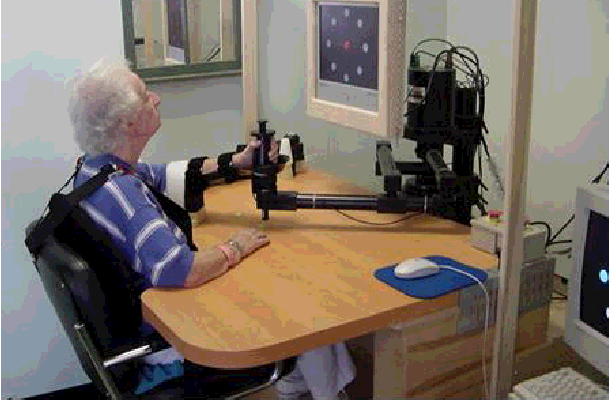
\includegraphics[scale=0.5]{images/background/MIT-MANUS.png}
    \caption[MIT-MANUS]{MIT-MANUS \cite{MIT-Manus}}
    \label{fig:my_label}
\end{figure}


Additionally, the \textbf{UL-EXO7} is a seven DoF robotic arm that provides assistive forces and a full range of motion shown in \autoref{fig:ULEXO7}. This robot, like the MIT-Manus, also is used to play an interactive game. The initial trial has been shown to have functional patient outcomes. 

\begin{figure}
    \centering
    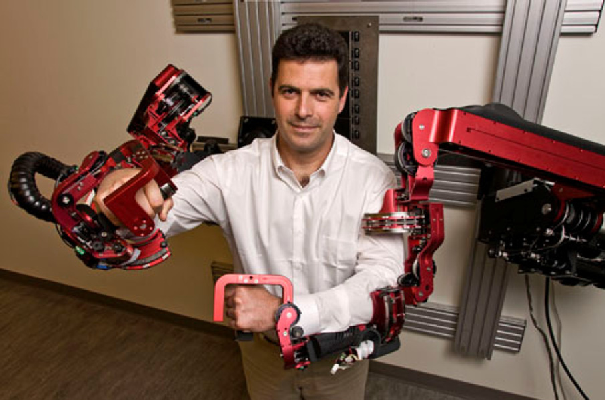
\includegraphics[scale=0.5]{images/background/ULEXO7.png}
    \caption[UL-EXO7]{UL-EXO7 \cite{byl2013chronic}}
    \label{fig:ULEXO7}
\end{figure}


Another rehabilitation arm exoskeleton is the \textbf{T-WREX}. Unlike some of the other systems, the T-WREX is pneumatically powered \cite{TWREX}; this had the advantage of large non-linear forces with low onboard mass. This system has also been shown to have successful rehabilitative outcomes \cite{housman2007arm}.
